% =====================================================================
%  GPSCrystalNet — geometry-aware crystal encoder (architecture figure)
% ---------------------------------------------------------------------
%  Standalone TikZ figure.  Narrative (left -> right):
%     (1) Crystal structure  ->  (2) Graph (geometry-aware)
%     ->  (3) Geometric featurization  ->  (4) GPS encoder (high level)
%  Emphasis is on the ENCODING side: how geometric information
%  (bonds, 3-body angles, coordination polyhedra) becomes model input.
%
%  Compile:
%     pdflatex gps_encoder.tex          (Overleaf: just hit Recompile)
%  Needs: tikz + the libraries below (texlive-pictures / texlive-latex-extra).
%  No pgfplots required — the RBF inset is drawn with plain TikZ \plot.
%
%  First draft: structure & content are settled; nudge coordinates to taste.
% =====================================================================
\documentclass[border=10pt]{standalone}
\usepackage{amsmath}
\usepackage{tikz}
\usetikzlibrary{positioning,arrows.meta,calc,fit,backgrounds,
                shapes.geometric,decorations.pathreplacing}

% ---- palette --------------------------------------------------------
\definecolor{Bcol}{HTML}{4C72B0}   % B-site / metal cation
\definecolor{Ocol}{HTML}{C44E52}   % anion (oxygen)
\definecolor{Acol}{HTML}{55A868}   % A-site large cation
\definecolor{panel}{HTML}{EEF1F6}  % light panel fill
\definecolor{accent}{HTML}{8172B3} % angle / geometric-emphasis colour
\definecolor{ink}{HTML}{2B2B2B}

% ---- shared styles --------------------------------------------------
\tikzset{
  atomB/.style={circle, draw=ink, thick, fill=Bcol,  minimum size=5.1mm,inner sep=0pt},
  atomO/.style={circle, draw=ink, thick, fill=Ocol,  minimum size=3.8mm,inner sep=0pt},
  atomA/.style={circle, draw=ink, thick, fill=Acol,  minimum size=6.8mm,inner sep=0pt},
  bond/.style={line width=1.8pt, gray!60!black},
  gbond/.style={line width=1.4pt, gray!55!black},
  polyedge/.style={line width=1.3pt, accent, dashed},
  angleArc/.style={line width=1.1pt, accent},
  stage/.style={-{Stealth[length=5mm,width=5mm]}, line width=3pt, gray!55},
  flow/.style={-{Stealth[length=3.5mm,width=3.5mm]}, line width=1.8pt, gray!60},
  annot/.style={-{Stealth[length=3mm]}, line width=1pt, accent, dashed},
  ebox/.style={draw=ink, rounded corners=2pt, fill=panel, align=center,
               font=\footnotesize, minimum width=36mm, minimum height=7mm,
               inner sep=3pt},
  subrow/.style={draw=ink, rounded corners=1.5pt, fill=white, align=center,
                 font=\scriptsize, minimum width=33mm, minimum height=6mm,
                 inner sep=2pt},
  container/.style={draw=ink, rounded corners=3pt, fill=accent!8, inner sep=4pt},
  pill/.style={draw=ink, very thick, rounded corners=6pt, fill=accent!18,
               align=center, font=\small\bfseries, minimum width=24mm,
               minimum height=8mm},
  ptitle/.style={font=\bfseries\sffamily, anchor=south},
  clbl/.style={font=\scriptsize\sffamily, text=ink},
}

% feature strip: #1=x  #2=y  #3=ncells  #4=fillcolor  (cell = 0.3 x 0.5)
\newcommand{\fvec}[4]{%
  \foreach \k in {1,...,#3}{%
    \draw[draw=ink, fill=#4]
      ({#1+0.3*(\k-1)},{#2}) rectangle ({#1+0.3*\k},{#2+0.5});}%
}

\begin{document}
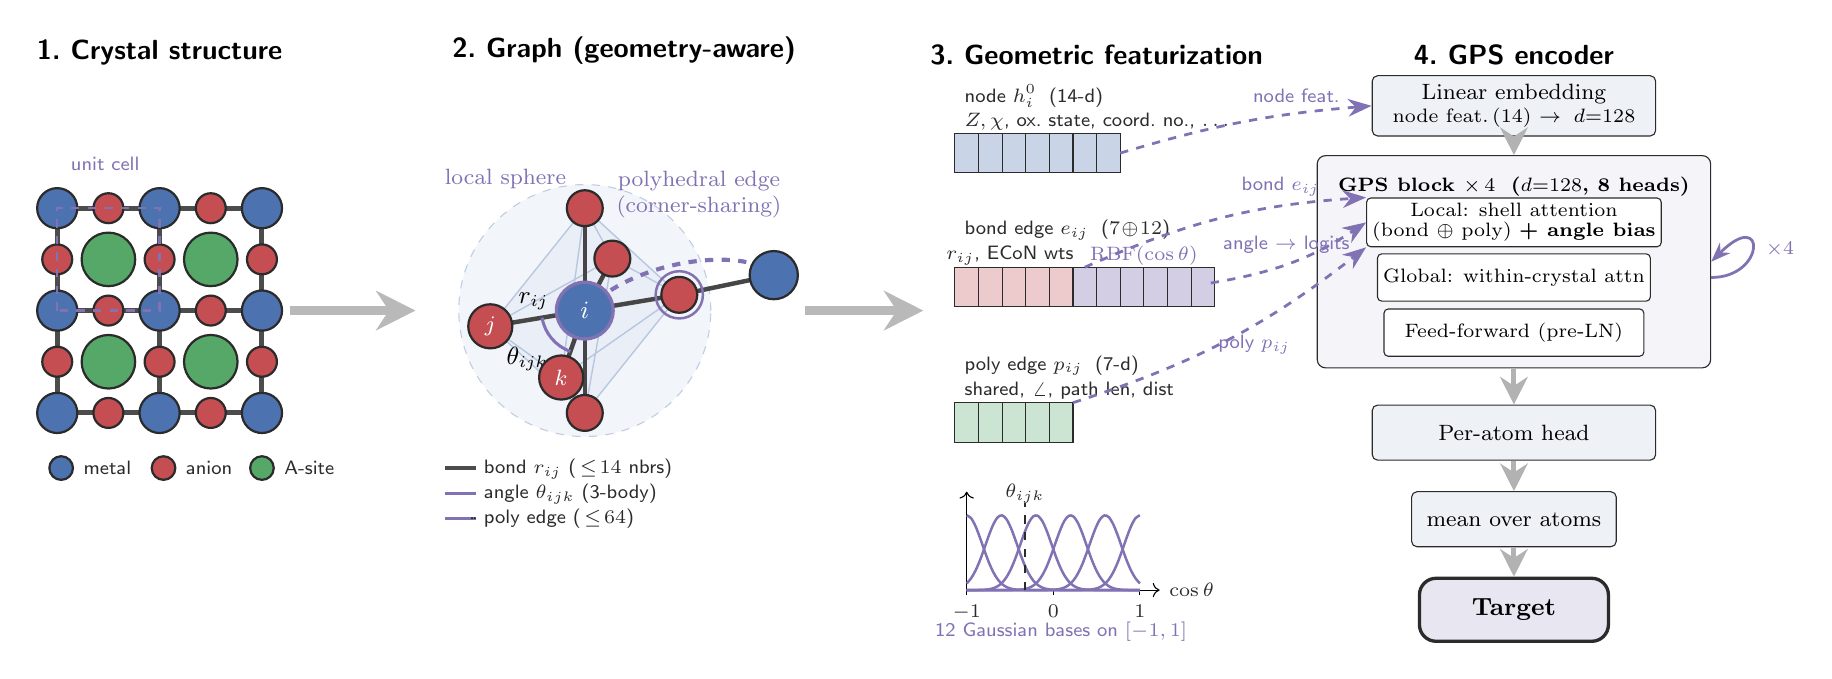
\begin{tikzpicture}[font=\sffamily]

% =====================================================================
%  OVERALL TITLE
% =====================================================================
%\node[font=\Large\bfseries, anchor=south] at (10.3,4.2)
%   {GPSCrystalNet: a geometry-aware crystal encoder};
%\node[font=\small\itshape, text=ink, anchor=north] at (10.3,4.1)
%   {formation-energy regression \,($E_\text{form}$ per atom)};

% =====================================================================
%  (1) CRYSTAL STRUCTURE  — perovskite-like slab (B-O network + A-sites)
% =====================================================================
\node[ptitle] at (1.3,3.0) {1.\ Crystal structure};
\begin{scope}[shift={(0,-1.3)}]   % centre the 2.6x2.6 block near y=0
  % B--O--B bonds (the O atoms sit on these on the midpoints)
  \foreach \j in {0,1,2}{ \draw[bond] (0,{1.3*\j}) -- (2.6,{1.3*\j}); }
  \foreach \i in {0,1,2}{ \draw[bond] ({1.3*\i},0) -- ({1.3*\i},2.6); }
  % A-site cations (large, behind)
  \foreach \p in {(0.65,0.65),(1.95,0.65),(0.65,1.95),(1.95,1.95)}{
     \node[atomA] at \p {}; }
  % B-site cations on the grid
  \foreach \i in {0,1,2}{ \foreach \j in {0,1,2}{
     \node[atomB] at ({1.3*\i},{1.3*\j}) {}; }}
  % O anions on the bond midpoints
  \foreach \p in {(0.65,0),(1.95,0),(0.65,1.3),(1.95,1.3),(0.65,2.6),(1.95,2.6),
                  (0,0.65),(0,1.95),(1.3,0.65),(1.3,1.95),(2.6,0.65),(2.6,1.95)}{
     \node[atomO] at \p {}; }
  % unit cell highlight (top-left cell) + label above the lattice
  \draw[dashed, thick, accent] (0,1.3) rectangle (1.3,2.6);
  \node[clbl, accent, anchor=south west] at (0.05,2.95) {unit cell};
\end{scope}
% mini legend (elements)
\begin{scope}[shift={(0.05,-2.0)}]
  \node[atomB, minimum size=3mm] (lb) at (0,0) {};
  \node[clbl, anchor=west] at (0.16,0) {metal};
  \node[atomO, minimum size=3mm] (lo) at (1.3,0) {};
  \node[clbl, anchor=west] at (1.46,0) {anion};
  \node[atomA, minimum size=3mm] (la) at (2.55,0) {};
  \node[clbl, anchor=west] at (2.71,0) {A-site};
\end{scope}

% ----- stage arrow 1 -> 2 -----
\draw[stage] (2.95,0) -- (4.55,0);

% =====================================================================
%  (2) GRAPH (geometry-aware)
% =====================================================================
\node[ptitle] at (7.2,3.0) {2.\ Graph (geometry-aware)};
\begin{scope}[shift={(4.9,0)},
              atomO/.append style={minimum size=4.56mm},
              atomB/.append style={minimum size=6.12mm},
              glbl/.style={font=\small, text=black}]   % bigger+darker in-graph labels
  % Perovskite BO6 (~20% larger): central B-site i octahedrally coordinated by
  % six O; the right-hand O is corner-shared with the next B-site (unlabeled).
  \coordinate (C)  at (1.8,0);       % center B-site i
  \coordinate (T)  at (1.8,1.3);     % apical O (top)
  \coordinate (Bo) at (1.8,-1.3);    % apical O (bottom)
  \coordinate (E1) at (3.0,0.2);     % equatorial O -- shared corner (right)
  \coordinate (E2) at (2.15,0.66);   % equatorial O (back)
  \coordinate (E3) at (0.6,-0.2);    % equatorial O (left)  -- j
  \coordinate (E4) at (1.5,-0.85);   % equatorial O (front) -- k
  \coordinate (Bnext) at (4.2,0.45); % next B-site, OUTSIDE the local sphere (moved right)

  % --- local sphere + coordination octahedron (background) ---
  \begin{scope}[on background layer]
     \fill[Bcol!7] (C) circle (1.6);
     \draw[Bcol!35, dashed] (C) circle (1.6);
     \fill[Bcol!12] (T) -- (E1) -- (Bo) -- (E3) -- cycle;        % silhouette
     \draw[Bcol!40, line width=0.5pt]
        (T) -- (E1) -- (Bo) -- (E3) -- cycle
        (E1) -- (E2) -- (E3) -- (E4) -- cycle                    % equatorial square
        (T) -- (E2) (Bo) -- (E2) (T) -- (E4) (Bo) -- (E4);       % front/back apex edges
  \end{scope}

  % --- graph edges (bonds): i bound to six O ---
  \foreach \o in {T,Bo,E1,E2,E3,E4}{ \draw[gbond, line width=1.6pt] (C) -- (\o); }
  \draw[gbond, line width=1.6pt] (E1) -- (Bnext);                % shared O -> next B-site
  % polyhedral 2nd-neighbour edge, arced high to stay clear of the bonds
  \draw[polyedge, line width=1.5pt]
       (C) .. controls (2.5,0.7) and (3.9,0.8) .. (Bnext);

  % --- bond angle  j--i--k  (two equatorial O neighbours: j=E3, k=E4) ---
  \draw[angleArc] ($(C)+(189.5:0.55)$) arc (189.5:250.6:0.55);
  \node[glbl] at (1.07,-0.61) {$\theta_{ijk}$};

  % --- atoms (j and k labelled inside their O atoms) ---
  \foreach \o in {T,E1,E2,Bo}{ \node[atomO] at (\o) {}; }
  \node[atomO, minimum size=5.6mm, font=\footnotesize, text=white] at (E3) {$j$};
  \node[atomO, minimum size=5.6mm, font=\footnotesize, text=white] at (E4) {$k$};
  \node[atomB] at (Bnext) {};
  \node[atomB, draw=accent, line width=1.2pt, minimum size=7.2mm,
        font=\small\bfseries, text=white] at (C) {$i$};
  \draw[accent, line width=0.9pt] (E1) circle (3.0mm);           % highlight shared O

  % --- labels (bigger + darker for readability) ---
  \node[glbl] at (1.15,0.12) {$r_{ij}$};                          % top-left, hugging the i--j edge
  \node[clbl, accent, font=\footnotesize, anchor=south west] at (-0.1,1.42) {local sphere};
  \node[clbl, accent, font=\footnotesize, align=center, anchor=south] at (3.25,1.05)
       {polyhedral edge\\(corner-sharing)};

  % small legend for the three geometric ingredients
  \node[clbl, anchor=north west] at (-0.1,-1.75) {%
     \begin{tabular}{@{}l@{\;}l@{}}
       \textcolor{gray!60!black}{\rule[0.4ex]{4mm}{1.6pt}} & bond $r_{ij}$ (\,$\le\!14$ nbrs)\\[1pt]
       \textcolor{accent}{\rule[0.4ex]{4mm}{1.1pt}} & angle $\theta_{ijk}$ (3-body)\\[1pt]
       \textcolor{accent}{\rule[0.4ex]{4mm}{1.1pt}}$\!\!\cdot\!\cdot$ & poly edge (\,$\le\!64$)\\
     \end{tabular}};
\end{scope}

% ----- stage arrow 2 -> 3 -----
\draw[stage] (9.5,0) -- (11.0,0);

% =====================================================================
%  (3) GEOMETRIC FEATURIZATION
% =====================================================================
\node[ptitle] at (13.2,3.0) {3.\ Geometric featurization};
\begin{scope}[shift={(11.4,0)}]
  % Each feature: name+dim on top line, contents on the line directly ABOVE its
  % strip; big gaps between blocks so each label group reads with its own cells.
  % --- node feature ---
  \node[clbl, anchor=west] at (0.0,2.72) {node $h_i^{0}$ \;(14-d)};
  \node[clbl, anchor=west] at (0.0,2.40)
     {\scriptsize $Z,\chi$, ox.\ state, coord.\ no., $\dots$};
  \fvec{0.0}{1.75}{7}{Bcol!30}
  \coordinate (nodecells) at (2.1,2.0);     % right edge of node strip -> embed

  % --- bond edge feature  (7 base  +  12 angle-RBF) ---
  \node[clbl, anchor=west] at (0.0,1.02) {bond edge $e_{ij}$ \;($7\!\oplus\!12$)};
  \node[clbl]         at (0.70,0.70) {\scriptsize $r_{ij}$, ECoN wts};
  \node[clbl, accent] at (2.40,0.70) {\scriptsize $\mathrm{RBF}(\cos\theta)$};
  \fvec{0.0}{0.05}{5}{Ocol!30}          % base geom: r, r/sumR, Voronoi, ECoN, dchi
  \fvec{1.5}{0.05}{6}{accent!35}        % angle block: RBF(cos theta)
  \coordinate (bondcells)  at (1.65,0.55);  % top of bond strip -> shell attention
  \coordinate (anglecells) at (3.25,0.35);  % right edge of angle cells -> attention logits

  % --- polyhedral edge feature ---
  \node[clbl, anchor=west] at (0.0,-0.70) {poly edge $p_{ij}$ \;(7-d)};
  \node[clbl, anchor=west] at (0.0,-1.02)
     {\scriptsize shared, $\angle$, path len, dist};
  \fvec{0.0}{-1.67}{5}{Acol!30}
  \coordinate (polycells) at (1.5,-1.17);   % top-right of poly strip -> shell attention

  % --- RBF(cos theta) inset curve ---
  \begin{scope}[shift={(0.15,-3.55)}]
    \draw[->] (0,0) -- (2.45,0) node[right,clbl]{$\cos\theta$};
    \draw[->] (0,0) -- (0,1.25);
    \foreach \tick/\lab in {0/-1,1.1/0,2.2/1}{
       \draw (\tick,0) -- (\tick,-0.06) node[below,clbl]{$\lab$}; }
    % a few Gaussian basis functions (centres span [-1,1] -> x in [0,2.2])
    \foreach \cx in {0.0,0.44,0.88,1.32,1.76,2.2}{
       \draw[accent, line width=0.9pt, smooth, domain=0:2.2, samples=40]
          plot (\x,{0.95*exp(-((\x-\cx)*(\x-\cx))/(2*0.2*0.2))}); }
    % current angle marker (e.g. ~109.5deg -> cos ~ -0.33 -> x ~ 0.74)
    \draw[ink, dashed] (0.74,0) -- (0.74,1.1);
    \node[clbl, ink] at (0.74,1.22) {$\theta_{ijk}$};
    \node[clbl, accent, anchor=north] at (1.2,-0.28)
       {12 Gaussian bases on $[-1,1]$};
  \end{scope}
\end{scope}

% (no single 3->4 stage arrow: the dashed routing arrows below show where
%  each feature actually enters the encoder)

% =====================================================================
%  (4) GPS ENCODER  (high level)
% =====================================================================
\node[ptitle] at (18.5,3.0) {4.\ GPS encoder};
\begin{scope}[shift={(16.8,0)}]
  % embedding
  \node[ebox] (embed) at (1.7,2.6)
       {Linear embedding\\[-1pt]\scriptsize node feat.\,(14) $\to\;d{=}128$};

  % GPS block internals (drawn first, container fitted behind)
  \node[font=\scriptsize\bfseries] (blktitle) at (1.7,1.58)
       {GPS block $\times\,4$ \;\scriptsize($d{=}128$, 8 heads)};
  \node[subrow] (local)  at (1.7,1.12)
       {Local: shell attention\\[-1pt](bond $\oplus$ poly) \textbf{+ angle bias}};
  \node[subrow] (global) at (1.7,0.42)
       {Global: within-crystal attn};
  \node[subrow] (ffn)    at (1.7,-0.28)
       {Feed-forward (pre-LN)};
  \begin{scope}[on background layer]
     \node[container, fit=(blktitle)(local)(global)(ffn)] (block) {};
  \end{scope}
  % "x4" recurrence hint
  \draw[-{Stealth[length=2.5mm]}, accent, line width=1pt]
       (block.east) ++(0,-0.2) .. controls +(0.7,0) and +(0.7,0.7) ..
       node[right=1pt,clbl,accent]{$\times 4$} (block.east);

  % head -> pool -> output
  \node[ebox] (head) at (1.7,-1.55)
       {Per-atom head};
  \node[ebox, minimum width=26mm] (mean) at (1.7,-2.65)
       {mean over atoms};
  \node[pill] (eform) at (1.7,-3.80) {Target};

  % vertical flow arrows (slimmer head so the gaps read clearly)
  \draw[flow] (embed.south)  -- (block.north);
  \draw[flow] (block.south)  -- (head.north);
  \draw[flow] (head.south)   -- (mean.north);
  \draw[flow] (mean.south)   -- (eform.north);
\end{scope}

% =====================================================================
%  cross-panel emphasis: angle features  ->  attention bias
% =====================================================================
\draw[annot] (anglecells) to[bend right=12]
     node[pos=0.46, above, clbl, accent]{angle $\to$ logits}
     (local.west);
% node features -> embedding;  bond & poly edges -> shell attention
\draw[annot] (nodecells) to[bend left=6]
     node[pos=0.72, above, clbl, accent]{node feat.} (embed.west);
\draw[annot] (bondcells) to[bend left=10]
     node[pos=0.72, above, clbl, accent]{bond $e_{ij}$} (local.north west);
\draw[annot] (polycells) to[bend right=10]
     node[pos=0.60, below, clbl, accent]{poly $p_{ij}$} (local.south west);

\end{tikzpicture}
\end{document}
